
\newpage

\titulo{Capítulos del compendio: Indicadores y sub-indicadores}


%\noindent\textbf{Recopilación:}

El Compendio Estadístico 2015 está organizado en siete capítulos: a) Población, b) disponibilidad de alimentos, c) acceso a los alimentos, d) consumo de los alimentos, e) utilización biológica de los alimentos, f) situación y atención a la desnutrición/malnutrición, e g) inversión pública en SAN. El primero reúne información sobre la caracterización de la población objeto de estudio; los siguientes cinco  capítulos están basados en los pilares de la seguridad alimentaria y nutricional; el séptimo capítulo busca explicar la situación de SAN en Guatemala (Figura \ref{figura3}). 

Como su nombre lo indica, el primer capítulo del Compendio sobre \textbf{población}, reúne información sobre la caracterización poblacional de Guatemala, incluyendo densidad poblacional, vivienda, pobreza y trabajo. 

El segundo capítulo del Compendio corresponde a garantizar la disponibilidad de una alimentación adecuada para todos: \textbf{dimensión de disponibilidad de alimentos. }Según la FAO (2015), es importante abordar el tema de la disponibilidad de alimentos adecuados, especialmente para los estratos más pobres de la sociedad. Asimismo, la producción agrícola debe ser ambiental, económica y socialmente sostenible, y debe garantizar la disponibilidad de alimentos suficientes para los que sufren las consecuencias de la inseguridad alimentaria y nutricional. Además, es importante asegurar la resiliencia de las comunidades y de los recursos naturales, incluyendo el mantenimiento de la diversidad genética.

Por otro lado, y según Coneval (2010), la disponibilidad de alimentos es el resultado de la producción interna, tanto de productos primarios como industrializados, del nivel de las reservas, importaciones y exportaciones, ayuda alimentaria y capacidad de almacenamiento y movilización. La disponibilidad debe ser estable, de forma que existan alimentos suficientes durante todo el año. Asimismo, debe ser adecuada a las condiciones sociales y culturales, y contar con productos sin sustancias dañinas para la salud.

El tercer capítulo se refiere a garantizar el acceso a una alimentación adecuada: \textbf{dimensión de acceso a los alimentos.} Las políticas para alcanzar esta meta van desde asegurar la cobertura de transferencias sociales a largo plazo, con base en el desarrollo de cadenas de valor, hasta enfrentar los desequilibrios comerciales y la volatilidad de los precios de los alimentos en mercados internacionales; esto último es un factor clave que afecta el acceso a alimentos nutritivos. Asimismo, se hace necesario enfrentar la integración de la producción de alimentos y el sistema de distribución, lo cual aumenta la propagación de alimentos de mala calidad (FAO, 2015).

En este sentido, los alimentos deben estar disponibles física y económicamente a toda la población. El acceso de alimentos saludables, así como su precio, dependen de la oferta y la demanda. La conducta del consumidor y sus preferencias pueden explicar las diferencias en los tipos de alimentos y la estructura de la oferta, así como las variaciones entre regiones con respecto a la disponibilidad de alimentos y la clase de establecimientos que los ofrecen. Además, el acceso económico de los hogares depende del ingreso y precio de los alimentos (Coneval, 2010).

El cuarto capítulo sobre la \textbf{dimensión de consumo de los alimentos}, se refiere a lo que consumen los miembros de cada hogar, ya sea que provenga de la autoproducción o del intercambio, ayudas o adquisiciones en los mercados, así como preparación y distribución intrafamiliar. El consumo es el resultado del poder de compra de los hogares y de quién realiza las compras y prepara los alimentos; además de hábitos y cultura, los cuales se pueden ver influidos por la publicidad y los medios de comunicación (Coneval, 2010). 

Asimismo, las elecciones de consumo de tipo de alimentos y de su estado (alimentos frescos, congelados, enlatados y preparados), dependen del tiempo que se tenga para obtener los ingredientes y preparar los alimentos. La limitación de tiempo es mayor en hogares con niños y cuando las mujeres trabajan fuera de la casa. Además, los individuos necesitan información sobre la elección de comida que hacen (Coneval, 2010).

El quinto capítulo, \textbf{dimensión de utilización biológica de los alimentos}, se refiere a que la desnutrición tiende a estar más concentrada en las poblaciones más vulnerables. Las políticas y programas de nutrición deben ser lo suficientemente amplios para enfrentar el retraso en el crecimiento y la deficiencia en micronutrientes (FAO, 2015). Asimismo, Coneval (2010) indica que el aprovechamiento biológico de los alimentos depende de las condiciones de salud del individuo, en particular del predominio de enfermedades infecciosas, así como de aspectos de saneamiento del medio; por ejemplo, el acceso a agua potable. Otros factores a tomar en cuenta son las condiciones del lugar, la forma de preparar los alimentos, y el consumo y almacenaje de los mismos que pueden contribuir a su contaminación (Coneval, 2010). 

\begin{figure}
	\centering
	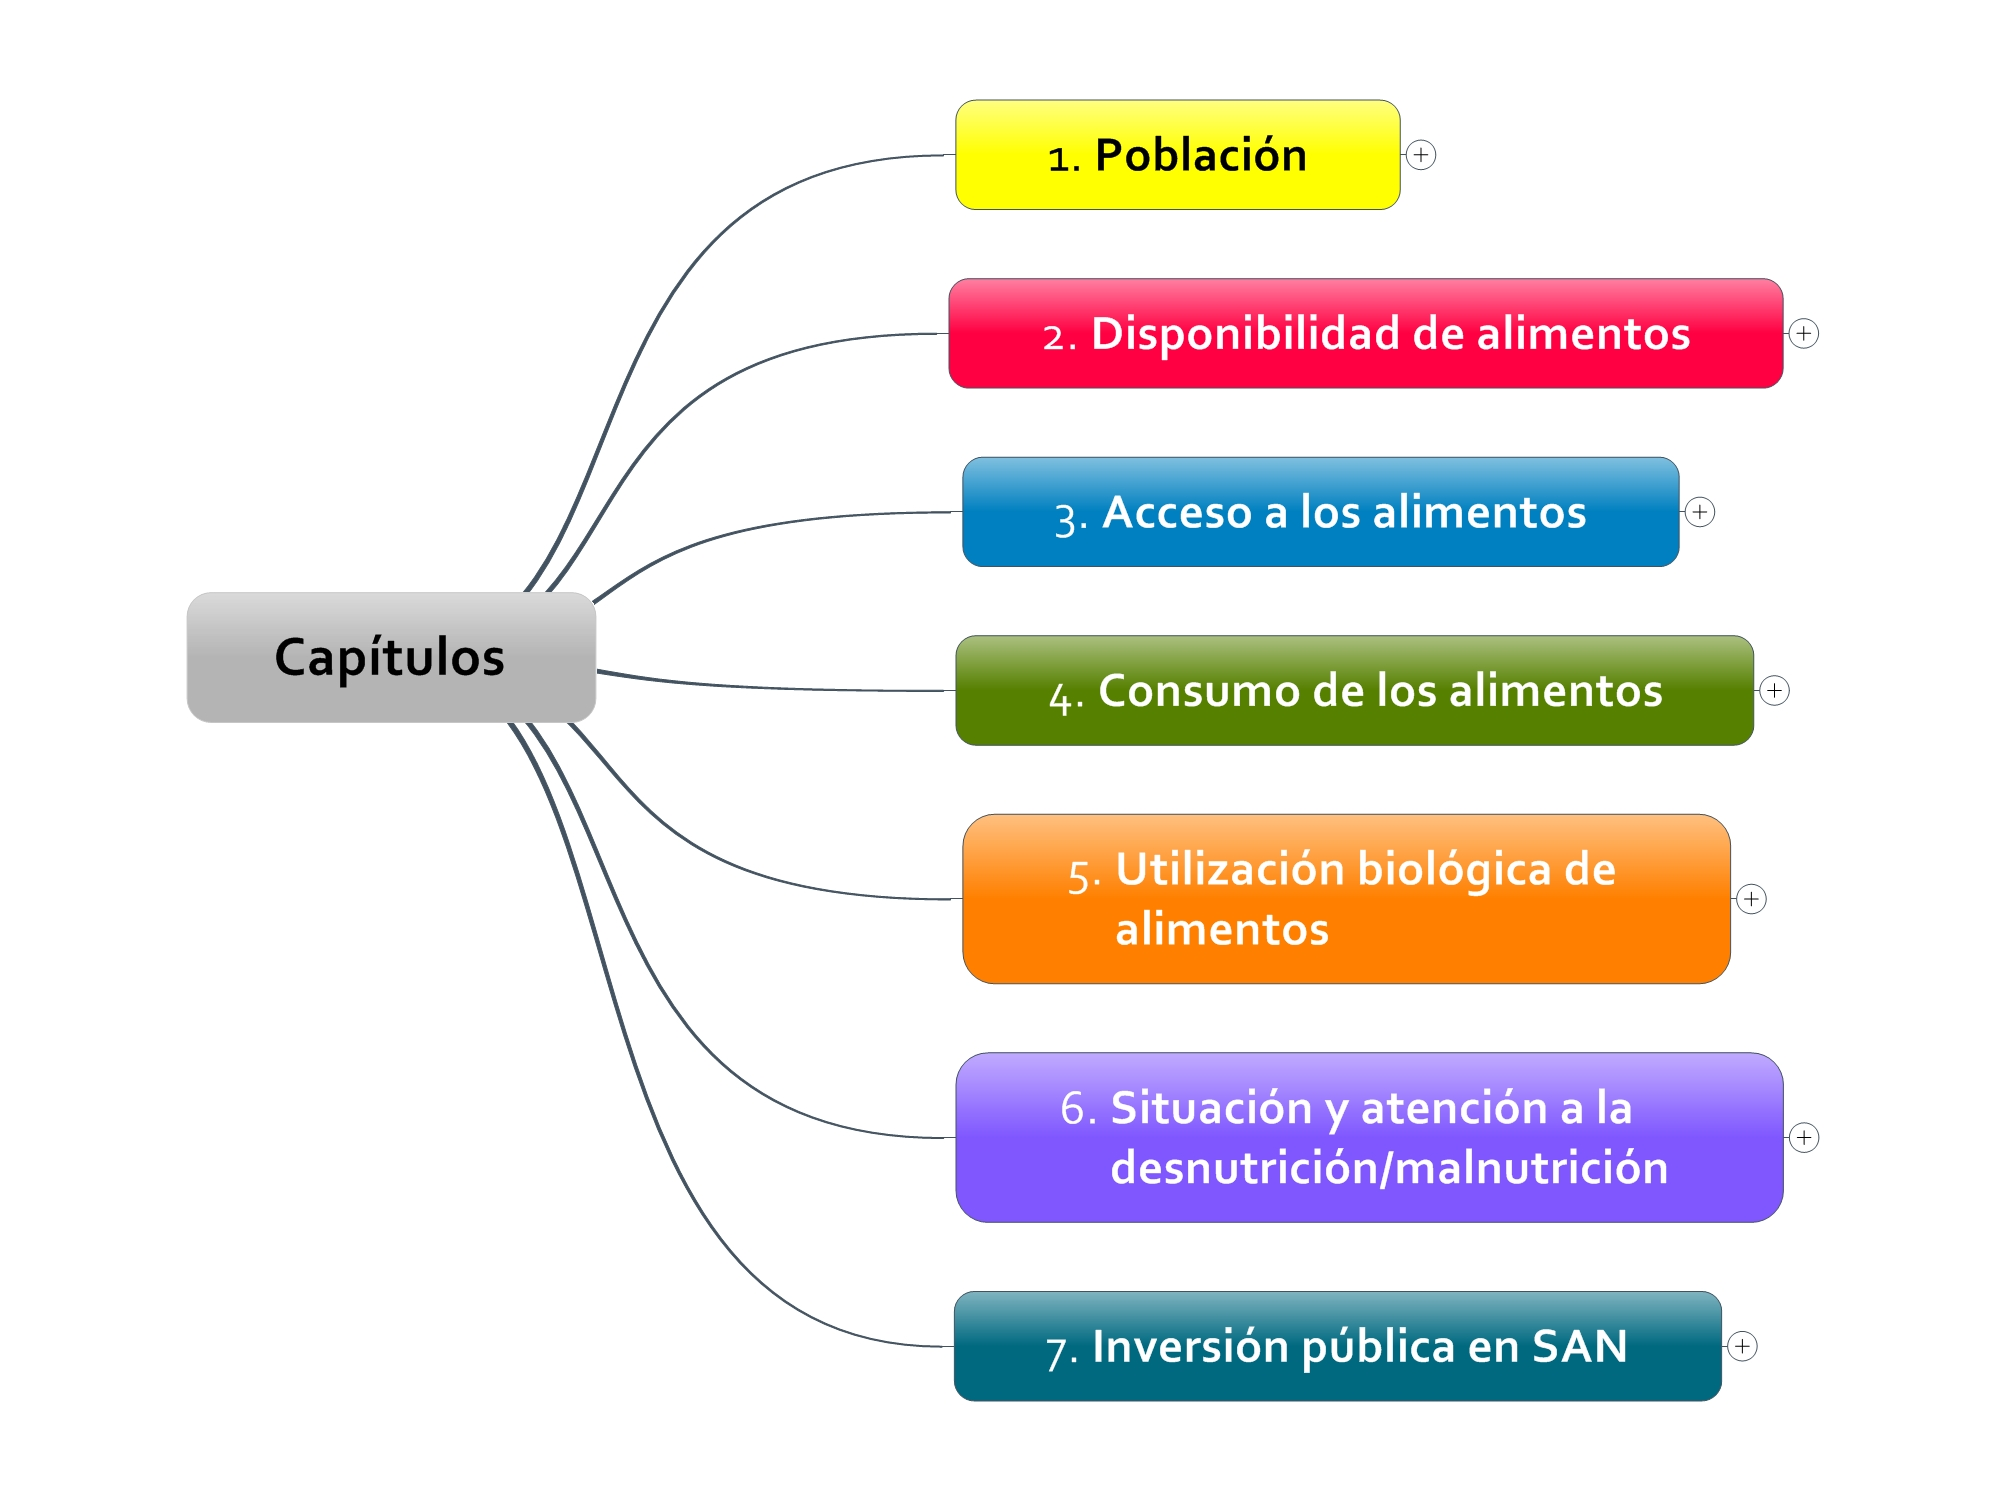
\includegraphics[width=0.7\textwidth]{Mapacap}
	\caption{Dimensiones/pilares que componen el Compendio Estadístico de Seguridad Alimentaria y Nutricional 2015. \textbf{Elaborado por:} Iarna-URL, 2015.}
	\label{figura3}
\end{figure}

El capítulo seis se refiere a la  \textbf{dimensión de la situación y atención a la desnutrición/malnutrición}. La desnutrición aguda, también conocida como emaciación o bajo peso para la talla, es causada por una ingesta insuficiente de alimentos y por la presencia de infecciones graves durante períodos prolongados. Por otro lado, la desnutrición crónica, también conocida como demedro o baja talla para la edad, es el retardo en el crecimiento lineal de los niños, como resultado de los efectos negativos acumulados de períodos de alimentación inadecuada, o por efectos fatales de infecciones agudas repetidas. Esta condición se presenta en los primeros tres años de vida, y sus consecuencias son irreversibles, ya que afectan negativamente el desarrollo motor, las funciones cognoscitivas y el desempeño escolar de los niños (Coneval, 2010). 

Por otro lado, también debe tomarse en cuenta la obesidad y el sobrepeso, los cuales son factores de riesgo para el desarrollo de enfermedades como diabetes, osteoartritis, enfermedades cardiovasculares, e incluso el desarrollo de ciertos tipos de cáncer, discapacidades o muerte prematura. De acuerdo con la Organización Mundial de la Salud (OMS), la obesidad y el sobrepeso se definen como la acumulación anormal o excesiva de grasa, la cual puede ser perjudicial para la salud, y que tiene como causa principal el desequilibrio entre la ingesta calórica y el consumo de energía (Coneval, 2010). Por último, se desarrolló una dimensión sobre la inversión pública en SAN, para describir los esfuerzos hechos en dicha materia mediante la implementación del Plan del Pacto Hambre Cero (PPH0).

El séptimo capítulo sobre la \textbf{inversión pública en SAN} en Guatemala, busca recopilar los logros en materia de SAN para el país en los últimos años.

Cada capítulo está dividido en una serie de indicadores y sub-indicadores elegidos para describir la situación de cada tema. Los indicadores fueron presentados en las reuniones de la Oficina Coordinadora Sectorial de Estadísticas de Seguridad Alimentaria y Nutricional (Ocsesan), y se le dio la oportunidad a los participantes de brindar su opinión sobre el listado de los mismos. Al final, no se tomaron en cuenta todos los indicadores disponibles, sino aquellos que se consideraron adecuados para que la información en el Compendio fuese útil y manejable.





\begin{landscape}
	
	\begin{figure}
		\centering
		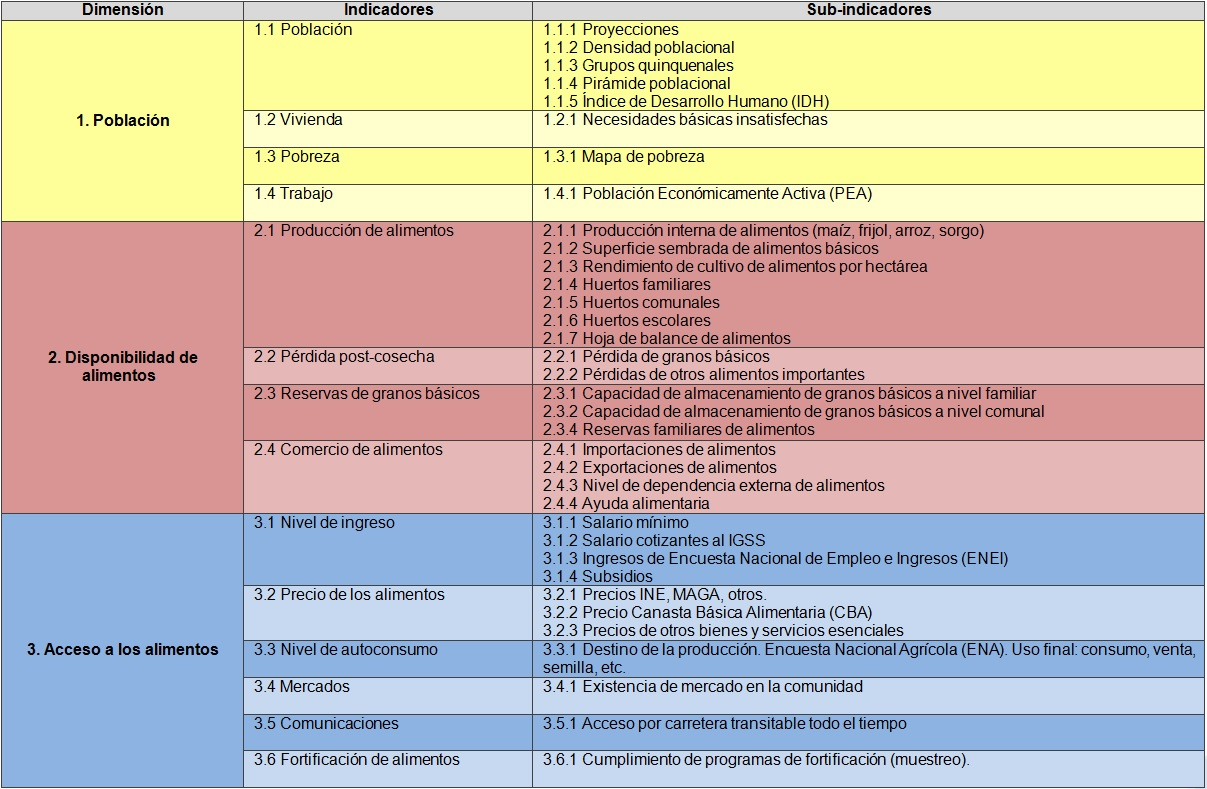
\includegraphics[width=1.4\textwidth]{cuadro1}
%		\caption{Dimensiones/pilares que componen el Compendio Estadístico de Seguridad Alimentaria y Nutricional 2015. \textbf{Elaborado por:} Iarna-URL, 2015.}
		\label{cuadro1}
	\end{figure}
\end{landscape}

\begin{landscape}
	
	\begin{figure}
		\centering
		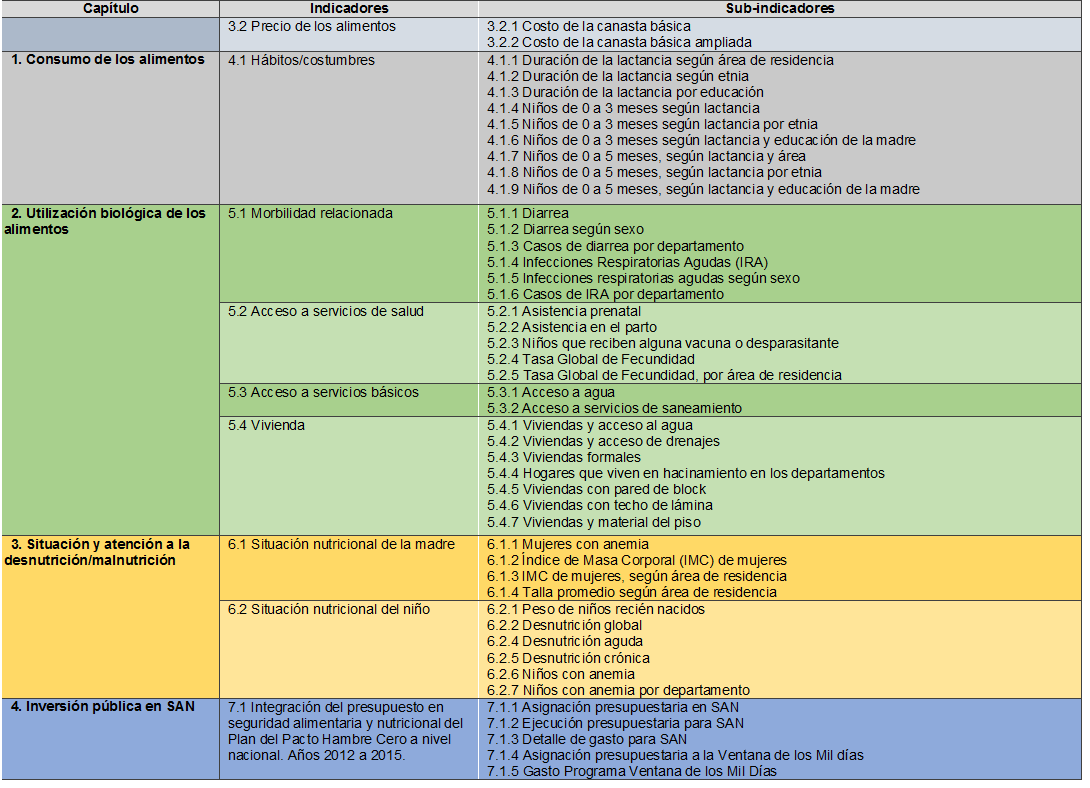
\includegraphics[width=1.4\textwidth]{cuadro2}
				\caption{Elaborado por: Iarna-URL, 2015.}
		\label{cuadro2}
	\end{figure}
\end{landscape}
